\section{Introduction}
This chapter describes the implementation of RV32ICore in VHDL, covering the structural organization of the design, the implementation of each major component, key design decisions made during development, and the toolchain used to compile and load test programs into the simulation environment. The implementation follows directly from the architecture described in Chapter 3, with each architectural unit realized as a distinct VHDL entity.    

\section{Design Philosophy}

The IDS is structured as a linear pipeline of independent modules, each consuming the same byte stream that flows from a physical interface receiver. Parsers at different protocol layers operate simultaneously on the same data; rule checkers fire one clock cycle after their corresponding parser completes. This means the system does not buffer a full packet before beginning inspection---field extraction and rule evaluation are interleaved with frame reception.

The choice of a byte-stream interface as the internal contract between modules makes each module independently testable and allows the physical reception mechanism to be swapped (from RMII simulation to AXI-Stream DMA for hardware) without modifying any parser or checker.

\section{Top-Level Structure}

The pipeline is wired together in a single top-level entity, \texttt{ids\_top.vhd}. It instantiates all sub-modules and connects them through internal signals. The byte stream---\texttt{rx\_byte}, \texttt{rx\_valid}, \texttt{rx\_sof}, \texttt{rx\_eof}---is broadcast to every parser simultaneously.

% --- FIGURE PLACEHOLDER ---
% Replace with the IDS pipeline diagram (Image 1 from your PNGs)
%
\begin{figure}[H]
	\centering
	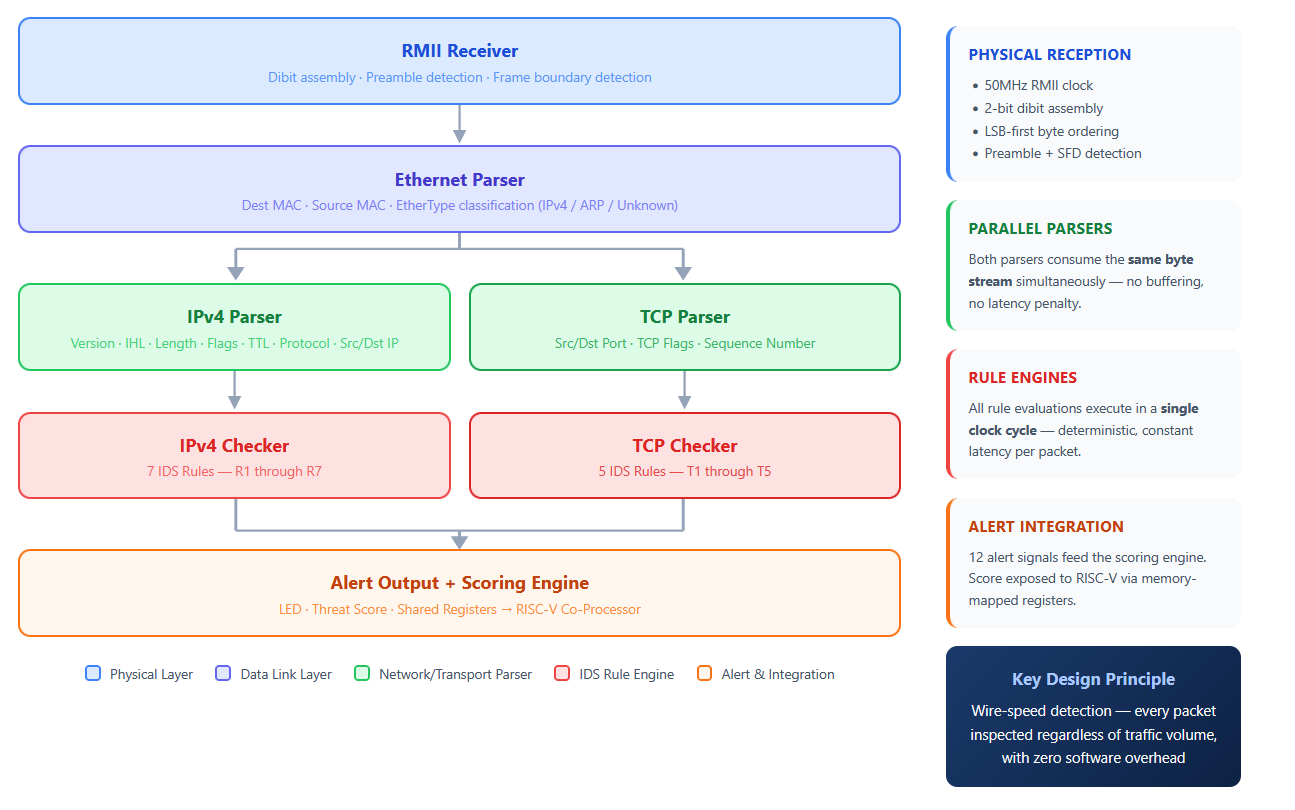
\includegraphics[width=0.95\textwidth]{ids_pipeline_diagram.png}
	\caption{IDS pipeline architecture showing parallel parsers and rule engines.}
	\label{fig:pipeline}
\end{figure}

\noindent The four-signal byte-stream interface carries the following semantics:
\begin{itemize}
	\item \texttt{rx\_sof} pulses for one clock cycle at the start of a new frame.
	\item \texttt{rx\_byte} / \texttt{rx\_valid} delivers one byte per clock when valid.
	\item \texttt{rx\_eof} pulses for one clock cycle at the end of the frame.
\end{itemize}

This interface is the internal standard across all modules.

\section{RMII Receiver (\texttt{rmii\_rx.vhd})}

In simulation, Ethernet frames are injected using RMII signalling: two data bits (a \emph{dibit}) are presented every clock cycle at 50\,MHz, LSB-first. The RMII receiver is a three-state FSM (IDLE, PREAMBLE, DATA) that assembles four consecutive dibits into one byte using a right-shift register:

\begin{lstlisting}[caption={Dibit assembly in \texttt{rmii\_rx.vhd}}, label=lst:rmii]
	shift_reg <= rmii_rxd & shift_reg(7 downto 2);
	if dibit_cnt = "11" then
	rx_byte  <= rmii_rxd & shift_reg(7 downto 2);
	rx_valid <= '1';
	end if;
\end{lstlisting}

The preamble state counts at least eight \texttt{01} dibits before accepting the Start Frame Delimiter (\texttt{11}). On hardware, this module is replaced by an AXI-Stream receiver that accepts bytes directly from the PS DMA engine; the rest of the pipeline is unchanged.

\section{Ethernet Parser (\texttt{eth\_parser.vhd})}

The Ethernet parser extracts the destination MAC, source MAC, and EtherType from the first 14 bytes of each frame. It uses a sequential FSM with states for each header field group (DST\_MAC, SRC\_MAC, ETHERTYPE, PAYLOAD, DONE). On the DONE state, it asserts \texttt{frame\_done} and one of \texttt{is\_ipv4}, \texttt{is\_arp}, or \texttt{is\_unknown} based on the EtherType value (0x0800, 0x0806, or other).

A key design decision is that all output signals default to \texttt{'0'} at the top of the clocked process and are only overridden in the DONE state. This prevents latches and ensures outputs are valid for exactly one clock cycle.

\section{Frame Counter (\texttt{frame\_counter.vhd})}

The frame counter accumulates per-second frame statistics (total, IPv4, ARP, unknown) using a hardware divider: a counter incremented every clock cycle triggers a \texttt{one\_sec\_tick} when it reaches \texttt{CLK\_FREQ\_HZ - 1}. On that tick, the running accumulators are latched to output registers and reset. This value is passed as a generic so the same code simulates at \texttt{CLK\_FREQ\_HZ = 1000} (1\,kHz) and synthesizes at \texttt{CLK\_FREQ\_HZ = 50\,000\,000} (50\,MHz), making testbenches fast without any code changes.

\section{IPv4 Parser (\texttt{ipv4\_parser.vhd})}

The IPv4 parser skips the 14-byte Ethernet header (counted in the ETH\_HEADER state) and then extracts the following fields from the IP header:

\begin{table}[H]
	\centering
	\caption{IPv4 header fields extracted by \texttt{ipv4\_parser.vhd}}
	\label{tab:ipv4fields}
	\begin{tabular}{lll}
		\toprule
		\textbf{Field} & \textbf{Byte offset} & \textbf{Width} \\
		\midrule
		Version / IHL   & 0      & 4 + 4 bits \\
		Total Length    & 2--3   & 16 bits    \\
		Flags / Fragment Offset & 6--7 & 3 + 13 bits \\
		TTL             & 8      & 8 bits     \\
		Protocol        & 9      & 8 bits     \\
		Source IP       & 12--15 & 32 bits    \\
		Destination IP  & 16--19 & 32 bits    \\
		\bottomrule
	\end{tabular}
\end{table}

The IHL field determines where the IP header ends (IHL\,$\times$\,4 bytes). The parser computes this boundary dynamically and transitions to WAIT\_EOF once all header bytes have been consumed, asserting \texttt{parse\_done} and \texttt{parse\_valid} (the latter only when \texttt{ip\_version = 4}) after the frame ends.

\section{IPv4 Checker (\texttt{ipv4\_checker.vhd})}

The IPv4 checker receives the parsed fields when \texttt{parse\_done} is asserted and evaluates all rules combinatorially inside a clocked process in a single clock cycle. A local variable \texttt{any\_alert} is OR'd across all rule conditions and drives the \texttt{alert\_any} output. Individual alert signals (\texttt{alert\_bad\_version}, \texttt{alert\_fragment}, etc.) are also driven, allowing the scoring engine to weight them differently.

\section{TCP Parser (\texttt{tcp\_parser.vhd})}

The TCP parser shares the same byte stream as the IPv4 parser. Because the TCP header begins at a byte offset that depends on the IP IHL field, the parser captures \texttt{ip\_ihl} and \texttt{ip\_protocol} from the IPv4 parser's output signals before the frame starts. It then skips to byte \texttt{14 + IHL\,$\times$\,4} (Ethernet header + IP header) before beginning TCP field extraction.

Fields extracted: source port, destination port, sequence number, and the flags byte. The flags byte at offset 13 of the TCP header encodes FIN, SYN, RST, PSH, ACK, and URG in bits 0--5.

\section{TCP Checker (\texttt{tcp\_checker.vhd})}

The TCP checker uses VHDL \texttt{alias} declarations to give readable names to individual flag bits:

\begin{lstlisting}[caption={Flag aliases in \texttt{tcp\_checker.vhd}}, label=lst:aliases]
	alias flag_fin : std_logic is tcp_flags(0);
	alias flag_syn : std_logic is tcp_flags(1);
	alias flag_rst : std_logic is tcp_flags(2);
\end{lstlisting}

Rules are expressed directly as Boolean conditions on these aliases, making the intent clear without bit-masking arithmetic.

\section{UDP Parser (\texttt{udp\_parser.vhd})}

The UDP header is 8 bytes long: source port (2), destination port (2), length (2), and checksum (2). The parser reuses the same skip-to-transport-layer logic as the TCP parser, activated only when \texttt{ip\_protocol = 0x11}. The \texttt{parse\_valid} output is asserted only for UDP packets.

\section{UDP Checker (\texttt{udp\_checker.vhd})}

The UDP checker evaluates nine rules on the extracted UDP fields and a configurable set of forbidden port values, shared with the TCP checker through the rule register bank.

% ============================================================
\section{Detection Rules}
\label{ch:rules}
% ============================================================

\subsection{Overview}

The IDS evaluates twenty detection rules across four protocol layers. Rules are grouped by the checker module that evaluates them. Each rule fires for exactly one clock cycle when its condition is met; the alert is latched and its weight added to the threat score.

\subsection{IPv4 Rules (R1--R12)}

\subsubsection{Rules R1--R7: Core Validity Checks}

These seven rules detect structurally malformed or trivially suspicious IPv4 packets.

\begin{table}[H]
	\centering
	\caption{IPv4 detection rules R1--R7}
	\label{tab:r1r7}
	\begin{tabular}{lll}
		\toprule
		\textbf{Rule} & \textbf{Condition} & \textbf{Attack / Anomaly} \\
		\midrule
		R1 & \texttt{ip\_version} $\neq$ 4          & Non-IPv4 / malformed packet \\
		R2 & \texttt{ip\_ihl} $<$ 5                  & Invalid header length       \\
		R3 & \texttt{ip\_length} $<$ 20              & Impossible packet size      \\
		R4 & \texttt{ip\_ttl} $\leq$ 1              & Suspicious TTL / traceroute \\
		R5 & \texttt{ip\_frag\_off} $>$ 0           & Fragmentation attack        \\
		R6 & \texttt{ip\_src} = \texttt{0.0.0.0}   & Spoofed source address      \\
		R7 & \texttt{ip\_src} = \texttt{ip\_dst}   & Land attack                 \\
		\bottomrule
	\end{tabular}
\end{table}

\subsubsection{Rules R8--R12: Bogon and Header Abuse}

These five rules detect packets whose source addresses belong to reserved or unroutable address blocks, or whose header fields abuse optional mechanisms.

\begin{table}[H]
	\centering
	\caption{IPv4 detection rules R8--R12}
	\label{tab:r8r12}
	\begin{tabular}{lll}
		\toprule
		\textbf{Rule} & \textbf{Condition} & \textbf{Attack / Anomaly} \\
		\midrule
		R8  & \texttt{ip\_src[31:24]} = \texttt{0x7F}          & Loopback source (127.x.x.x)        \\
		R9  & \texttt{ip\_src[31:16]} = \texttt{0xA9FE}        & Link-local source (169.254.x.x)    \\
		R10 & \texttt{ip\_src[31:28]} = \texttt{0xE}           & Multicast source (224--239.x.x.x) \\
		R11 & \texttt{ip\_ihl} $>$ 5                           & IP options present                  \\
		R12 & \texttt{ip\_flags[2]} = \texttt{'1'}             & Reserved IPv4 flag bit set          \\
		\bottomrule
	\end{tabular}
\end{table}

Rules R8--R10 share a single enable bit (\texttt{bogon\_check\_en}) in the rule register bank so the RISC-V can disable them all at once on a network segment where such addresses may legitimately appear.

\subsection{TCP Rules (T1--T5)}

\begin{table}[H]
	\centering
	\caption{TCP detection rules T1--T5}
	\label{tab:t1t5}
	\begin{tabular}{lll}
		\toprule
		\textbf{Rule} & \textbf{Condition} & \textbf{Attack / Anomaly} \\
		\midrule
		T1 & SYN = 1 and FIN = 1                    & Illegal flag combination    \\
		T2 & SYN = 1 and RST = 1                    & Illegal flag combination    \\
		T3 & All flags = \texttt{0x00}              & NULL scan (port probe)      \\
		T4 & All flags = \texttt{0xFF}              & XMAS scan (port probe)      \\
		T5 & \texttt{dst\_port} $\in$ forbidden set & Access to forbidden service \\
		\bottomrule
	\end{tabular}
\end{table}

The forbidden port set (rule T5) is stored in configurable registers and defaults to Telnet (23), FTP (21), and TFTP (69). The RISC-V processor can update these values without reprogramming the FPGA.

\subsection{UDP Rules (U1--U9)}

\begin{table}[H]
	\centering
	\caption{UDP detection rules U1--U9}
	\label{tab:u1u9}
	\begin{tabular}{lp{6cm}p{6cm}}
		\toprule
		\textbf{Rule} & \textbf{Condition} & \textbf{Attack / Anomaly} \\
		\midrule
		U1 & \texttt{udp\_dst\_port} $\in$ forbidden set & Access to forbidden UDP service \\
		U2 & \texttt{udp\_length} $<$ 8 & Invalid UDP length field \\
		U3 & \texttt{udp\_length} $=$ 0 & Completely malformed UDP packet \\
		U4 & \texttt{udp\_src\_port} $\in$ \{53, 123, 11211, 19\} & Amplification attack response (DNS/NTP/Memcached/CHARGEN) \\
		U5 & \texttt{ip\_src} $=$ \texttt{ip\_dst} $\wedge$ \texttt{udp\_src\_port} $=$ \texttt{udp\_dst\_port} & UDP land attack \\
		U6 & \texttt{udp\_length} $>$ 1472 & Oversized datagram (exceeds Ethernet MTU) \\
		U7 & \texttt{udp\_src\_port} $=$ 0 $\vee$ \texttt{udp\_dst\_port} $=$ 0 & Reserved port zero used \\
		U8 & \texttt{udp\_dst\_port} $=$ 1900 & SSDP/UPnP abuse \\
		U9 & \texttt{udp\_dst\_port} $=$ 11211 & Memcached amplification request \\
		\bottomrule
	\end{tabular}
\end{table}
\newpage
\subsection{Alert Weighting}

Each alert type is assigned a weight, and the scoring engine accumulates weights additively. The RISC-V classifies traffic into three severity tiers based on the accumulated score.
\begin{table}[H]
	\centering
	\caption{Alert weights used by the scoring engine}
	\label{tab:weights}
	\begin{tabular}{llr}
		\toprule
		\textbf{Alert} & \textbf{Rule} & \textbf{Weight} \\
		\midrule
		Bad version          & R1       & 5  \\
		Bad IHL              & R2       & 5  \\
		Bad length           & R3       & 10 \\
		Low TTL              & R4       & 5  \\
		Fragmentation        & R5       & 15 \\
		Spoofed source       & R6       & 20 \\
		Land attack          & R7       & 25 \\
		Bogon source         & R8--R10  & 15 \\
		IP options           & R11      & 10 \\
		Reserved flag        & R12      & 10 \\
		SYN+FIN              & T1       & 25 \\
		SYN+RST              & T2       & 20 \\
		NULL scan            & T3       & 20 \\
		XMAS scan            & T4       & 20 \\
		Forbidden TCP port   & T5       & 15 \\
		Forbidden UDP port   & U1       & 15 \\
		Malformed UDP length & U2, U3   & 10 \\
		Amplification resp.  & U4       & 20 \\
		UDP land attack      & U5       & 25 \\
		Oversized UDP        & U6       & 10 \\
		Port zero            & U7       & 10 \\
		SSDP/UPnP abuse      & U8       & 15 \\
		Memcached amplif.    & U9       & 20 \\
		\bottomrule
	\end{tabular}
\end{table}

The score decays by a configurable rate every second when no new alerts fire, preventing a historical event from permanently elevating the severity level.